\documentclass[12pt]{article}
  \usepackage{geometry}
 \usepackage[round]{natbib}
 \usepackage{graphicx}
 \geometry{a4paper}
  \usepackage[T1]{fontenc}
  \usepackage[utf8]{inputenc}
  \usepackage{authblk}
  \usepackage[running]{lineno}
  \usepackage{setspace}
  \usepackage{booktabs}
  \usepackage{tabularx}
  \usepackage{chngpage}
  \usepackage{amsmath}
  \usepackage{amssymb}
  \usepackage[hidelinks]{hyperref}
 \usepackage[textsize=tiny]{todonotes}
\usepackage{pdfpages, caption}
\usepackage{listings}
\usepackage{minted}
\usepackage{framed}
\usepackage{mdframed}
\usepackage[section]{placeins}

\usepackage{natbib} %package for bibliography

\renewcommand{\thefigure}{S\arabic{figure}}
\renewcommand{\thetable}{S\arabic{table}}
\renewcommand{\thesection}{S\arabic{section}}


\newenvironment{problem}[2][Problem]{\begin{trivlist}
		\item[\hskip \labelsep {\bfseries #1}\hskip \labelsep {\bfseries #2.}]}{\end{trivlist}}

\DeclareMathOperator*{\argmax}{arg\,max}

\renewcommand\listingscaption{Stan code}
\definecolor{apricot}{rgb}{0.984,0.81,0.69}
\BeforeBeginEnvironment{minted}{\begin{mdframed}[backgroundcolor=apricot]}
	\AfterEndEnvironment{minted}{\end{mdframed}}
\newcommand{\Lim}[1]{\raisebox{0.5ex}{\scalebox{0.8}{$\displaystyle \lim_{#1}\;$}}}
\newcommand*\widefbox[1]{\fbox{\hspace{2em}#1\hspace{2em}}}
\interfootnotelinepenalty=10000

\usepackage{framed}
\makeatletter
\newenvironment{kframe}{%
	\def\at@end@of@kframe{}%
	\ifinner\ifhmode%
	\def\at@end@of@kframe{\end{minipage}}%
\begin{minipage}{\columnwidth}%
	\fi\fi%
	\def\FrameCommand##1{\hskip\@totalleftmargin \hskip-\fboxsep
		\colorbox{shadecolor}{##1}\hskip-\fboxsep
		% There is no \\@totalrightmargin, so:
		\hskip-\linewidth \hskip-\@totalleftmargin \hskip\columnwidth}%
	\MakeFramed {\advance\hsize-\width
		\@totalleftmargin\z@ \linewidth\hsize
		\@setminipage}}%
{\par\unskip\endMakeFramed%
	\at@end@of@kframe}
\makeatother

\definecolor{fgcolor}{rgb}{0.345, 0.345, 0.345}
\newcommand{\hlnum}[1]{\textcolor[rgb]{0.686,0.059,0.569}{#1}}%
\newcommand{\hlstr}[1]{\textcolor[rgb]{0.192,0.494,0.8}{#1}}%
\newcommand{\hlcom}[1]{\textcolor[rgb]{0.678,0.584,0.686}{\textit{#1}}}%
\newcommand{\hlopt}[1]{\textcolor[rgb]{0,0,0}{#1}}%
\newcommand{\hlstd}[1]{\textcolor[rgb]{0.345,0.345,0.345}{#1}}%
\newcommand{\hlkwa}[1]{\textcolor[rgb]{0.161,0.373,0.58}{\textbf{#1}}}%
\newcommand{\hlkwb}[1]{\textcolor[rgb]{0.69,0.353,0.396}{#1}}%
\newcommand{\hlkwc}[1]{\textcolor[rgb]{0.333,0.667,0.333}{#1}}%
\newcommand{\hlkwd}[1]{\textcolor[rgb]{0.737,0.353,0.396}{\textbf{#1}}}%

\definecolor{orangeBright}{RGB}{243,146,0}
\definecolor{blueBright}{RGB}{54,169,225}
\definecolor{pinkBright}{RGB}{214,11,82}
\definecolor{shadecolor}{rgb}{.97, .97, .97}
\definecolor{messagecolor}{rgb}{0, 0, 0}
\definecolor{warningcolor}{rgb}{1, 0, 1}
\definecolor{errorcolor}{rgb}{1, 0, 0}
\newenvironment{knitrout}{}{} % an empty environment to be redefined in TeX


\usepackage{xr}
\externaldocument{figures}
\externaldocument{supplementary_materials_methods}

%   \doublespacing
% \raggedright
\title{A Meta-analysis of Longevity Estimates of Mosquito Vectors of Disease: Supplementary Figures}
\author{Ben Lambert, Ace North, Charles Godfray}

\begin{document}
\maketitle

\section{MRR experments}
Figures \ref{fig:mrr_lifeSpanVsRange} and \ref{fig:mrr_lifeSpanVsTrapDensity} show the estimates of lifespan versus the trapping range and spatial density of traps at study location. In these cases, the lifespans shown were obtained from the non-hierarchical model with the exponential survival model. The spatial density of traps was obtained assuming that the study area was a circular area of radius equal to the maximum trapping distance.

Fig. \ref{fig:mrr_female_blood_sugar} shows the lifespans obtained for each pre-release feeding category for each genus and across all studies using the hierarchical Bayesian model with exponential survival model. In the genus-level models, the feeding-specific effects (not pre-fed, blood-fed-only and sugar-fed-only) were estimated as independent random effects for each genus with standard normal priors. For the overall model, the feeding-specific effects were estimated as independent random effects across all studies, with a standard normal prior.

\begin{table}[htbp]
	\begin{tabular}{l|l|l|l|l|l|l|l|l}
		\textbf{Genus} & \textbf{Species} & \textbf{5$\%$} & \textbf{25$\%$} & \textbf{50$\%$} & \textbf{75$\%$} & \textbf{95\%} &  \textbf{Mean} & \textbf{Std. dev.}\\
		\hline
		\textit{Aedes} & \textit{simpsoni s.l.} & 6.3 & 11.3 & 18.3 & 31.8 & 75.0 & 26.9 & 29.5 \\
		\textit{Aedes} & \textit{communis} & 10.0 & 13.2 & 15.4 & 18.2 & 24.3 & 16.2 & 5.2 \\
		\textit{Anopheles} & \textit{koliensis} & 6.7 & 10.5 & 15.2 & 24.0 & 56.5 & 21.9 & 25.2 \\
		\textit{Anopheles} & \textit{punctulatus} & 7.2 & 10.7 & 15.1 & 22.8 & 48.9 & 20.3 & 28.6 \\
		\textit{Aedes} & \textit{cantans} & 9.7 & 12.0 & 13.9 & 16.1 & 20.6 & 14.4 & 4.7 \\
		\textit{Aedes} & \textit{albopictus} & 8.0 & 10.0 & 11.6 & 13.7 & 17.7 & 12.1 & 3.4 \\
		\textit{Anopheles} & \textit{albimanus} & 5.9 & 8.6 & 11.6 & 16.9 & 35.7 & 15.2 & 18.7 \\
		\textit{Anopheles} & \textit{darlingi} & 4.9 & 7.3 & 10.2 & 16.0 & 37.5 & 14.5 & 14.8 \\
		\textit{Anopheles} & \textit{maculatus} & 5.7 & 7.9 & 10.2 & 13.7 & 24.3 & 12.2 & 8.7 \\
		\textit{Anopheles} & \textit{culicifacies s.l.} & 4.6 & 7.3 & 9.1 & 11.4 & 18.2 & 10.1 & 6.9 \\
		\textit{Anopheles} & \textit{sergenti} & 3.6 & 5.9 & 8.7 & 13.8 & 32.6 & 12.4 & 13.4 \\
		\textit{Aedes} & \textit{triseriatus} & 5.6 & 6.6 & 7.5 & 8.5 & 10.7 & 7.7 & 1.8 \\
		\textit{Anopheles} & \textit{farauti s.l.} & 4.2 & 5.4 & 6.4 & 7.7 & 10.5 & 6.8 & 2.1 \\
		\textit{Aedes} & \textit{africanus} & 3.4 & 5.1 & 6.2 & 7.8 & 11.9 & 7.0 & 9.3 \\
		\textit{Aedes} & \textit{aegypti} & 2.8 & 4.5 & 6.2 & 8.5 & 13.9 & 7.0 & 3.8 \\
		\textit{Culex} & \textit{quinquefasciatus} & 4.3 & 5.2 & 5.9 & 7.0 & 9.4 & 6.3 & 1.8 \\
		\textit{Culex} & \textit{nigripalpus} & 3.5 & 4.6 & 5.8 & 7.5 & 11.3 & 6.4 & 3.1 \\
		\textit{Aedes} & \textit{notoscriptus} & 2.9 & 4.0 & 5.4 & 8.2 & 20.2 & 7.9 & 9.5 \\
		\textit{Culex} & \textit{pipiens} & 3.4 & 4.4 & 5.2 & 6.4 & 9.0 & 5.6 & 2.0 \\
		\textit{Anopheles} & \textit{saperoi} & 3.5 & 4.2 & 4.9 & 5.8 & 8.2 & 5.2 & 2.0 \\
		\textit{Anopheles} & \textit{gambiae s.l.} & 3.0 & 3.8 & 4.4 & 5.1 & 6.4 & 4.5 & 1.1 \\
		\textit{Aedes} & \textit{melanimon} & 3.3 & 3.9 & 4.3 & 4.8 & 5.7 & 4.4 & 1.0 \\
		\textit{Anopheles} & \textit{funestus s.l.} & 2.9 & 3.6 & 4.2 & 4.8 & 6.0 & 4.3 & 1.0 \\
		\textit{Anopheles} & \textit{lesteri} & 2.4 & 3.2 & 3.9 & 5.0 & 7.5 & 4.4 & 2.1 \\
		\textit{Anopheles} & \textit{quadrimaculatus} & 3.3 & 3.6 & 3.9 & 4.2 & 4.8 & 4.0 & 0.5 \\
		\textit{Anopheles} & \textit{pseudopunctipennis s.l.} & 2.3 & 2.9 & 3.5 & 4.3 & 6.7 & 3.8 & 1.9 \\
		\textit{Aedes} & \textit{vexans} & 1.9 & 2.3 & 2.6 & 3.0 & 4.1 & 2.8 & 1.0 \\
		\textit{Culex} & \textit{tarsalis} & 1.9 & 2.1 & 2.3 & 2.4 & 2.7 & 2.3 & 0.3 \\
		\textit{Anopheles} & \textit{vestitipennis} & 1.3 & 1.8 & 2.2 & 2.9 & 4.4 & 2.5 & 1.2 \\
		\textit{Anopheles} & \textit{albitarsis s.l.} & 1.3 & 1.6 & 1.9 & 2.2 & 2.9 & 2.0 & 1.0 \\
		\textit{Culex} & \textit{tritaeniorhynchus} & 0.7 & 0.9 & 1.1 & 1.2 & 1.6 & 1.1 & 1.0 \\
		\textit{Anopheles} & \textit{subpictus s.l.} & 0.4 & 0.6 & 0.8 & 1.1 & 2.4 & 1.1 & 2.6 \\
		\hline
		\textit{Aedes} & \text{} & 2.8 & 4.8 & 6.9 & 10.0 & 17.2 & 8.1 & 4.9 \\
		\textit{Anopheles} & \text{} & 1.5 & 3.0 & 5.0 & 8.4 & 17.8 & 6.8 & 6.4 \\
		\textit{Culex} & \text{} & 1.1 & 1.8 & 2.5 & 3.5 & 5.6 & 2.9 & 1.5 \\
		\hline
		\textbf{Overall} & \text{} & 1.4 & 2.8 & 4.6 & 7.5 & 15.4 & 6.0 & 5.2 \\
	\end{tabular}
	\caption{\textbf{Posterior summaries of mean unfed female mosquito lifespan from the MRR analysis.} The 5\%, 25\%, 50\%, 75\% and 95\% columns indicate the respective quantiles of the posterior distribution for mean lifespan, and the `Mean' and `Std. dev.' columns indicate the posterior mean and standard deviation of mean lifespan.}
	\label{tab:mrr_estimated_lifespans}%
\end{table}%


\begin{figure}[h]
	\centerline{\includegraphics[width=1\textwidth]{./Figure_files/mrr_genus_vs_species_vs_top.pdf}}
	\caption{\textbf{The estimated predictive accuracy of the species- and overall-level models relative to the genus-level model.} The predictive accuracy was determined using K-Fold cross-validation as described in SOM; the measure of accuracy presented here by the central dots is the difference in estimated expected log pointwise predictive density compared to the exponential model. The lower and upper whiskers represent the lower and upper bounds of the 95\% confidence interval in predictive accuracy.}
	\label{fig:mrr_genusTopLevel}
\end{figure}

\begin{figure}[h]
	\centerline{\includegraphics[width=1\textwidth]{./Figure_files/mrr_lifeSpanVsRange.pdf}}
	\caption{\textbf{Posterior estimates of mean mosquito lifespan for each time-series versus the trapping range.} The markers show the median posterior estimates, with the lower and upper bounds indicating the 25\% and 75\% quantiles, respectively. The black line shows a linear regression line estimated using the median posterior lifetimes, with the grey shading indicating 95\% confidence intervals. All estimates were obtained using the non-hierarchical exponential survival model.}
	\label{fig:mrr_lifeSpanVsRange}
\end{figure}

\begin{figure}[h]
	\centerline{\includegraphics[width=1\textwidth]{./Figure_files/mrr_lifespanVsTrapDensity.pdf}}
	\caption{\textbf{Posterior estimates of mean mosquito lifespan for each time-series versus the trap density.} The markers show the median posterior estimates, with the lower and upper bounds indicating the 25\% and 75\% quantiles, respectively. The trap density was estimated assuming traps were contained within a circular area with radius equal to the trapping range. The black line shows a linear regression line estimated using the median posterior lifetimes, with the grey shading indicating 95\% confidence intervals. All estimates were obtained using the non-hierarchical exponential survival model.}
	\label{fig:mrr_lifeSpanVsTrapDensity}
\end{figure}

\begin{figure}[h]
	\centerline{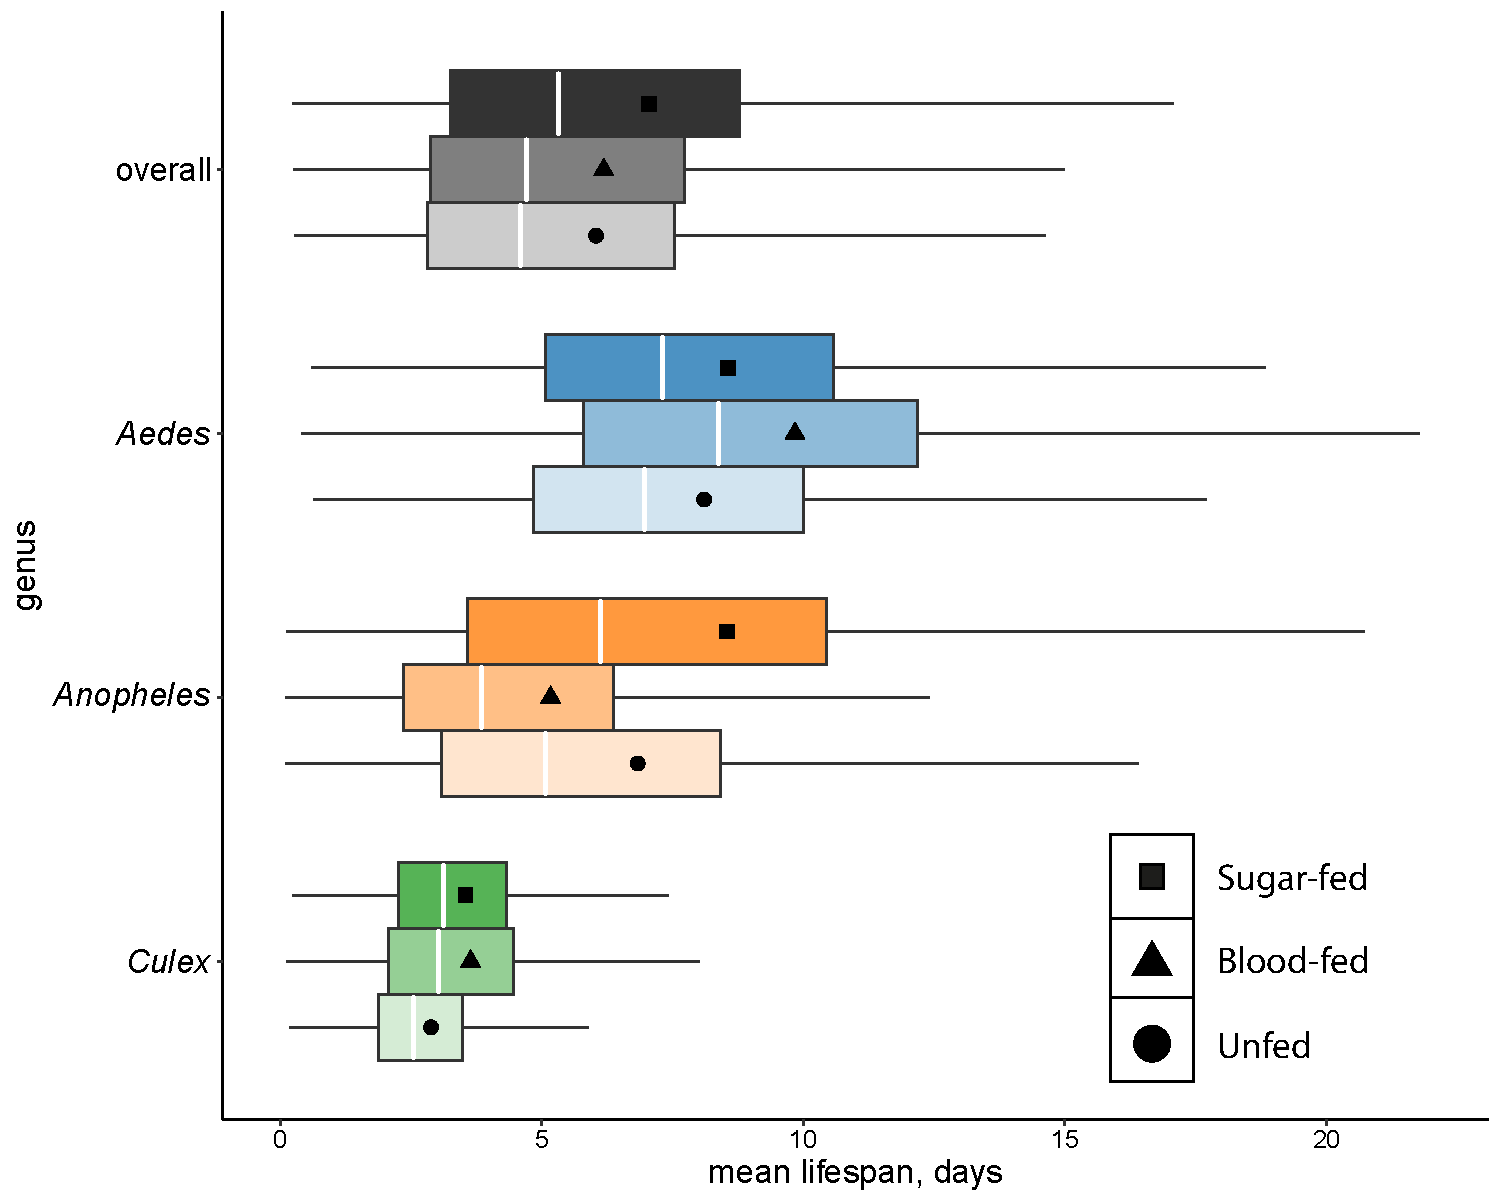
\includegraphics[width=1\textwidth]{./Figure_files/mrr_female_blood_sugar.pdf}}
	\caption{\textbf{Posterior estimates of female mosquito mean lifespan according to pre-release feeding status across species, genus and overall groupings as determined from the MRR data.} The lifespans shown are for mosquitoes that were not fed with sugar or blood (for females) before release. The middle line in each box shows the median estimates and the solid dot indicates the mean. The left and right box edges show the 25\%, and 75\% posterior quantiles respectively. The whiskers show the range of the data, excluding points lying more than 1.5 times the interquartile range away from each edge of the box. The numbers before the start of the left whisker indicate the number of individual time-series within each species. All estimates were obtained using the hierarchical exponential survival model.}
	\label{fig:mrr_female_blood_sugar}
\end{figure}

\begin{figure}[h]
	\centerline{\includegraphics[width=1\textwidth]{./Figure_files/mrr_lifeSpanVsTemperature.pdf}}
	\caption{\textbf{Posterior estimates of mean mosquito lifespan for each time-series versus the average monthly temperature for each study location and date.} The markers show the median posterior estimates, with the lower and upper bounds indicating the 25\% and 75\% quantiles, respectively. The black line shows a regression line with linear and quadratic terms estimated using the median posterior lifetimes, with the grey shading indicating 95\% confidence intervals. All estimates of lifespan were obtained using the non-hierarchical exponential survival model.}\label{fig:mrr_temperature}
\end{figure}

\begin{figure}[h]
	\centerline{\includegraphics[width=1\textwidth]{./Figure_files/mrr_ThreeSpeciesVersusTemperature.pdf}}
	\caption{\textbf{Posterior estimates of mean mosquito lifespan for each time-series versus the average monthly temperature for the four species with the most data.} The markers show the median posterior estimates, with the lower and upper bounds indicating the 25\% and 75\% quantiles, respectively. The black line shows a regression line with linear and quadratic terms estimated using the median posterior lifetimes, with the grey shading indicating 95\% confidence intervals. All estimates of lifespan were obtained using the non-hierarchical exponential survival model.}\label{fig:mrr_ThreeSpeciesVersusTemperature}
\end{figure}

\section{Dissection analysis}

\begin{figure}[h]
	\centerline{\includegraphics[width=1.3\textwidth]{./Figure_files/dissection_individualEstimates_allSpecies.pdf}}
	\caption{\textbf{Individual time-series estimates of adult mosquito mean lifespan ordered by species median as determined from the dissection data.} The middle line in each box shows the median estimates. The left and right box whiskers show the 25\%, and 75\% posterior quantiles respectively. All estimates were obtained using the non-hierarchical exponential survival model.}
	\label{fig:dissection_individualEstimates_allSpecies}
\end{figure}

\begin{table}[htbp]
	\begin{tabular}{l|l|l|l|l|l|l|l|l}
		\textbf{Genus} & \textbf{Species} & \textbf{5$\%$} & \textbf{25$\%$} & \textbf{50$\%$} & \textbf{75$\%$} & \textbf{95\%} &  \textbf{Mean} & \textbf{Std. dev.}\\
		\hline
		\textit{Anopheles} & \textit{sergentii} & 1.0 & 1.9 & 2.5 & 3.4 & 6.2 & 3.0 & 2.5 \\
		\textit{Anopheles} & \textit{gambiae s.l.} & 0.7 & 1.2 & 1.9 & 2.9 & 5.4 & 2.4 & 1.9 \\
		\textit{Culex} & \textit{thalassius} & 1.1 & 1.6 & 1.8 & 2.1 & 2.9 & 1.9 & 1.0 \\
		\textit{Anopheles} & \textit{farauti s.l.} & 1.5 & 1.6 & 1.7 & 1.7 & 1.9 & 1.7 & 0.1 \\
		\textit{Anopheles} & \textit{minimus} & 0.7 & 1.2 & 1.7 & 2.2 & 4.1 & 2.0 & 2.2 \\
		\textit{Anopheles} & \textit{maculipennis} & 0.8 & 1.1 & 1.4 & 1.8 & 2.9 & 1.6 & 0.7 \\
		\textit{Culex} & \textit{pipiens} & 1.1 & 1.3 & 1.4 & 1.5 & 1.7 & 1.4 & 0.2 \\
		\textit{Mansonia} & \textit{uniformis} & 0.9 & 1.1 & 1.1 & 1.2 & 1.4 & 1.1 & 0.2 \\
		\textit{Anopheles} & \textit{rivulorum} & 0.8 & 1.0 & 1.1 & 1.1 & 1.4 & 1.1 & 0.2 \\
		\textit{Anopheles} & \textit{melas} & 0.8 & 1.0 & 1.0 & 1.1 & 1.3 & 1.0 & 0.2 \\
		\textit{Anopheles} & \textit{culicifacies} & 0.9 & 1.0 & 1.0 & 1.1 & 1.2 & 1.0 & 0.1 \\
		\textit{Anopheles} & \textit{subpictus} & 0.6 & 0.9 & 1.0 & 1.2 & 2.1 & 1.2 & 2.0 \\
		\textit{Aedes} & \textit{aegypti} & 0.5 & 0.8 & 1.0 & 1.2 & 2.0 & 1.2 & 3.0 \\
		\textit{Anopheles} & \textit{quadrimaculatus} & 0.7 & 0.9 & 1.0 & 1.1 & 1.3 & 1.0 & 0.2 \\
		\textit{Anopheles} & \textit{stephensi} & 0.6 & 0.8 & 1.0 & 1.1 & 1.6 & 1.0 & 0.4 \\
		\textit{Anopheles} & \textit{darlingi} & 0.7 & 0.8 & 0.9 & 1.0 & 1.3 & 1.0 & 0.2 \\
		\textit{Culex} & \textit{quinquefasciatus} & 0.4 & 0.7 & 0.9 & 1.3 & 2.2 & 1.1 & 0.6 \\
		\textit{Aedes} & \textit{polynesiensis} & 0.8 & 0.9 & 0.9 & 0.9 & 1.0 & 0.9 & 0.1 \\
		\textit{Culex} & \textit{tritaeniorhynchus} & 0.3 & 0.6 & 0.9 & 1.3 & 4.2 & 2.5 & 30.8 \\
		\textit{Culex} & \textit{annulirostris} & 0.5 & 0.8 & 0.9 & 1.0 & 1.4 & 0.9 & 0.5 \\
		\textit{Aedes} & \textit{samoanus} & 0.6 & 0.7 & 0.8 & 0.9 & 1.0 & 0.8 & 0.2 \\
		\textit{Aedes} & \textit{sollicitans} & 0.4 & 0.5 & 0.6 & 0.8 & 1.3 & 0.7 & 0.5 \\
		\textit{Aedes} & \textit{vexans} & 0.4 & 0.5 & 0.6 & 0.7 & 0.9 & 0.6 & 0.7 \\
		\textit{Anopheles} & \textit{cruzii} & 0.3 & 0.5 & 0.5 & 0.7 & 1.1 & 0.6 & 0.4 \\
		\textit{Anopheles} & \textit{bellator} & 0.3 & 0.4 & 0.5 & 0.6 & 1.0 & 0.6 & 1.8 \\
		\hline
		\textit{Anopheles} & \textit{} & 0.6 & 1.0 & 1.4 & 1.9 & 3.2 & 1.6 & 0.9 \\
		\textit{Mansonia} & \textit{} & 0.9 & 1.1 & 1.1 & 1.2 & 1.4 & 1.1 & 0.2 \\
		\textit{Culex} & \textit{} & 0.5 & 0.8 & 1.0 & 1.4 & 2.3 & 1.2 & 0.6 \\
		\textit{Aedes} & \textit{} & 0.6 & 0.7 & 0.8 & 0.9 & 1.1 & 0.8 & 0.2 \\
		\hline
		\textbf{Overall} & \textit{} & 0.5 & 0.8 & 1.2 & 1.7 & 2.7 & 1.3 & 0.7 \\
	\end{tabular}
	\caption{\textbf{Posterior summaries of mean female mosquito lifespan in terms of gonotrophic cycles from dissection studies.} The 5\%, 25\%, 50\%, 75\% and 95\% columns indicate the respective quantiles of the posterior distribution for mean lifespan, and the `Mean' and `Std. dev.' columns indicate the posterior mean and standard deviation of mean lifespan.}
	\label{tab:dissection_estimated_lifespans}%
\end{table}

\begin{figure}[ht]
	\centerline{\includegraphics[width=1\textwidth]{./Figure_files/gonotrophic_data.pdf}}
	\caption{\textbf{Raw gonotrophic cycle duration estimates for A. the 1st cycle and B. subsequent cycles.} When present, the confidence intervals represent our estimates of the 95\% confidence interval on gonotrophic cycle duration (see Section \ref{sec:dissection_gonotrophicMethod} for a discussion of how we handle this issue); if our estimate of the lower limit was below zero, we deemed this unbiological and set it to 1 day for this graph. If no statement of uncertainty was given in the estimates then we indicate this by a triangle marker. The studies are ordered within each Genus according to the central estimate of gonotrophic duration.}\label{fig:dissection_gonotrophicCycleRaw}
\end{figure}



\begin{figure}[h]
	\centerline{\includegraphics[width=1\textwidth]{./Figure_files/dissection_lifetimes_exponential_chron.pdf}}
	\caption{\textbf{Posterior estimates of female mosquito mean chronological lifespan across species, genus and overall groupings as determined from the dissection data.} The lifespans shown are for mosquitoes that were not fed with sugar or blood (for females) before release. The middle line in each box shows the median estimates and the solid dot indicates the mean. The left and right box edges show the 25\%, and 75\% posterior quantiles respectively. The whiskers show the range of the data, excluding points lying more than 1.5 times the interquartile range away from each edge of the box. The numbers before the start of the left whisker indicate the number of individual time-series within each species. All estimates were obtained using the hierarchical exponential survival model.}
	\label{fig:dissection_lifetimes_exponential_chron}
\end{figure}

\begin{table}[htbp!]
	\begin{tabular}{l|l|l|l|l|l|l|l|l}
		\textbf{Genus} & \textbf{Species} & \textbf{5$\%$} & \textbf{25$\%$} & \textbf{50$\%$} & \textbf{75$\%$} & \textbf{95\%} &  \textbf{Mean} & \textbf{Std. dev.}\\
		\hline
	\textit{Culex} & \textit{thalassius} & 5.7 & 8.2 & 9.4 & 11.0 & 15.6 & 10.1 & 5.2 \\
	\textit{Anopheles} & \textit{sergentii} & 3.7 & 6.4 & 8.5 & 11.5 & 20.6 & 10.1 & 8.1 \\
	\textit{Culex} & \textit{pipiens} & 5.7 & 6.6 & 7.2 & 7.8 & 8.9 & 7.2 & 1.0 \\
	\textit{Anopheles} & \textit{gambiae s.l.} & 2.4 & 4.3 & 6.4 & 9.8 & 18.3 & 8.0 & 6.3 \\
	\textit{Anopheles} & \textit{farauti s.l.} & 4.8 & 5.5 & 5.9 & 6.3 & 6.9 & 5.9 & 0.6 \\
	\textit{Anopheles} & \textit{minimus} & 2.7 & 4.4 & 5.8 & 7.7 & 13.7 & 6.9 & 8.1 \\
	\textit{Anopheles} & \textit{maculipennis} & 2.8 & 4.0 & 5.1 & 6.4 & 9.6 & 5.5 & 2.3 \\
	\textit{Culex} & \textit{quinquefasciatus} & 2.0 & 3.4 & 4.8 & 6.9 & 11.7 & 5.6 & 3.3 \\
	\textit{Aedes} & \textit{aegypti} & 2.3 & 3.7 & 4.7 & 5.6 & 9.3 & 5.6 & 12.3 \\
	\textit{Culex} & \textit{annulirostris} & 2.7 & 3.9 & 4.6 & 5.4 & 7.5 & 4.9 & 2.4 \\
	\textit{Culex} & \textit{tritaeniorhynchus} & 1.6 & 3.2 & 4.6 & 7.2 & 22.8 & 13.0 & 174.0 \\
	\textit{Mansonia} & \textit{uniformis} & 3.4 & 4.0 & 4.4 & 4.9 & 5.5 & 4.5 & 0.7 \\
	\textit{Aedes} & \textit{polynesiensis} & 3.2 & 3.7 & 4.1 & 4.5 & 5.1 & 4.1 & 0.6 \\
	\textit{Anopheles} & \textit{rivulorum} & 2.8 & 3.4 & 3.8 & 4.2 & 5.0 & 3.9 & 0.7 \\
	\textit{Anopheles} & \textit{melas} & 2.8 & 3.3 & 3.7 & 4.1 & 4.8 & 3.8 & 0.7 \\
	\textit{Anopheles} & \textit{culicifacies s.l.} & 2.8 & 3.3 & 3.7 & 4.1 & 4.7 & 3.7 & 0.6 \\
	\textit{Anopheles} & \textit{subpictus s.l.} & 2.2 & 3.1 & 3.7 & 4.5 & 7.0 & 4.3 & 6.6 \\
	\textit{Aedes} & \textit{samoanus} & 2.7 & 3.2 & 3.6 & 4.0 & 4.9 & 3.7 & 1.0 \\
	\textit{Anopheles} & \textit{quadrimaculatus} & 2.4 & 3.1 & 3.5 & 4.0 & 4.8 & 3.6 & 0.8 \\
	\textit{Anopheles} & \textit{stephensi} & 2.1 & 2.9 & 3.5 & 4.2 & 5.7 & 3.7 & 1.5 \\
	\textit{Anopheles} & \textit{darlingi} & 2.3 & 2.9 & 3.4 & 3.8 & 4.7 & 3.4 & 0.9 \\
	\textit{Aedes} & \textit{sollicitans} & 1.6 & 2.3 & 2.9 & 3.6 & 6.1 & 3.3 & 2.5 \\
	\textit{Aedes} & \textit{vexans} & 1.7 & 2.2 & 2.7 & 3.1 & 4.2 & 3.0 & 3.3 \\
	\textit{Anopheles} & \textit{cruzii} & 1.2 & 1.6 & 2.0 & 2.5 & 4.0 & 2.2 & 1.3 \\
	\textit{Anopheles} & \textit{bellator} & 1.0 & 1.4 & 1.7 & 2.1 & 3.6 & 2.1 & 5.4 \\
		\hline
		\textit{Culex} & \textit{} & 2.5 & 4.0 & 5.4 & 7.6 & 12.3 & 6.2 & 3.2 \\
		\textit{Anopheles} & \textit{} & 2.1 & 3.6 & 4.9 & 6.8 & 10.8 & 5.5 & 2.9 \\
		\textit{Mansonia} & \textit{} & 3.3 & 4.0 & 4.5 & 4.9 & 5.6 & 4.5 & 0.8 \\
		\textit{Aedes} & \textit{} & 2.5 & 3.3 & 3.8 & 4.3 & 5.2 & 3.8 & 0.9 \\
		\hline
		\textit{Overall} & \textit{} & 2.0 & 3.3 & 4.7 & 6.4 & 10.2 & 5.2 & 2.6 \\
	\end{tabular}
	\caption{\textbf{Posterior summaries of mean female mosquito lifespan in terms of chronological time from dissection studies.} The 5\%, 25\%, 50\%, 75\% and 95\% columns indicate the respective quantiles of the posterior distribution for mean lifespan, and the `Mean' and `Std. dev.' columns indicate the posterior mean and standard deviation of mean lifespan.}
	\label{tab:dissection_estimated_lifespans_chron}%
\end{table}

\subsection{Comparison of LBLs between the MRR and dissection analyses}
To conduct a comparison between the LBLs from the MRR analysis and from the dissections, we converted the latter lifespans from gonotrophic cycles to chronological age as described in Section \ref{sec:dissection_conversion}. We conducted ANOVA using the individual time series estimates of LBL for each of the 10 species with estimates from both MRR- and dissection-based analysis. The results of this analysis are shown in Table \ref{tab:comparison}.

\begin{table}[htbp]
	\centering
	\begin{tabular}{l|l|l|l|l}
		species & \multicolumn{1}{l}{$\text{df}_1$} & \multicolumn{1}{l}{$\text{df}_2$} & \multicolumn{1}{l}{F} & \multicolumn{1}{l}{p} \\
		\midrule
		\textit{Ae. aegypti} & 1     & 55    & 1.9   & 0.17 \\
		\textit{A. culicifacies s.l.} & 1     & 19    & 2.2   & 0.15 \\
		\textit{A. darlingi} & 1     & 6     & 80.7   & 0.00 \\
		\textit{An. farauti s.l.} & 1     & 14    & 2.1  & 0.17 \\
		\textit{A. gambiae s.l.} & 1     & 37    & 4.3   & 0.05 \\
		\textit{Cx. pipiens} & 1     & 13    & 0.4   & 0.56 \\
		\textit{A. quadrimaculatus} & 1     & 8     & 2.2     & 0.18 \\
		\textit{Cx. quinquefasciatus} & 1     & 13    & 2.2    & 0.16 \\
		\textit{A. sergentii} & 1     & 8     & 1.0    & 0.36 \\
		\textit{A. subpictus} & 1     & 2    & 11.4   & 0.08 \\
		\textit{Cx. tritaeniorhynchus} & 1     & 5     & 3.6   & 0.12 \\
		\textit{Ae. vexans} & 1     & 2     & 1.1   & 0.41 \\
	\end{tabular}%
	\caption{\textbf{The results of comparisons between LBLs for those species with data for MRRs and dissection-based studies.} The ANOVA tests were conducted using median posterior LBLs estimated at the time-series level.}
	\label{tab:comparison}%
\end{table}%

\section{Detinova parity analysis}

\begin{table}[htbp!]
\begin{tabular}{l|l|l|l|l|l|l|l|l}
	\textbf{Genus} & \textbf{Species} & \textbf{5$\%$} & \textbf{25$\%$} & \textbf{50$\%$} &
	\textbf{75$\%$} & \textbf{95$\%$} & \textbf{Mean} & \textbf{Std. dev.} \\
	\hline
	\textit{Anopheles} & \textit{funestus} & 4.9 & 8.1 & 11.9 & 18.7 & 43.8 & 19.0 & 70.6 \\
	\textit{Anopheles} & \textit{funestus s.l.} & 4.4 & 7.7 & 13.0 & 25.6 & 88.0 & 31.6 &
	\text{$>$100} \\
	\textit{Anopheles} & \textit{nili s.l.} & 5.6 & 8.9 & 12.3 & 17.7 & 36.2 & 17.1 & 41.5 \\
	\textit{Anopheles} & \textit{gambiae} & 4.0 & 6.1 & 8.4 & 12.1 & 23.1 & 10.4 & 7.9 \\
	\textit{Anopheles} & \textit{gambiae (Form M)} & 2.9 & 5.2 & 8.2 & 14.0 & 42.3 &
	\text{$>$100} & \text{$>$100} \\
	\textit{Anopheles} & \textit{arabiensis} & 3.2 & 4.9 & 7.1 & 11.1 & 23.8 & 9.8 & 10.6 \\
	\textit{Anopheles} & \textit{gambiae s.l.} & 3.5 & 5.7 & 8.7 & 14.6 & 36.4 & 13.2 & 16.2 \\
	\textit{Anopheles} & \textit{leucosphyrus} & 5.0 & 8.2 & 11.3 & 15.9 & 31.6 & 28.2 &
	\text{$>$100} \\
	\textit{Anopheles} & \textit{leucosphyrus s.l.} & 4.5 & 7.8 & 11.1 & 15.8 & 33.7 & 19.0 &
	\text{$>$100} \\
	\textit{Anopheles} & \textit{aconitus} & 2.3 & 5.2 & 9.4 & 17.5 & \text{$>$100} &
	\text{$>$100} & \text{$>$100} \\
	\textit{Anopheles} & \textit{dirus (Sp. A)} & 4.9 & 7.5 & 10.3 & 15.1 & 28.6 & 13.0
	& 10.3 \\
	\textit{Anopheles} & \textit{dirus s.l.} & 4.2 & 6.6 & 9.2 & 14.0 & 29.9 & 12.3 & 12.5 \\
	\textit{Anopheles} & \textit{barbirostris s.l.} & 2.4 & 5.2 & 8.6 & 16.5 & \text{$>$100} &
	\text{$>$100} & \text{$>$100} \\
	\textit{Anopheles} & \textit{minimus (Sp. A)} & 3.1 & 6.2 & 10.2 & 18.1 & 79.2 &
	88.5 & \text{$>$100} \\
	\textit{Anopheles} & \textit{minimus s.l.} & 3.9 & 5.8 & 7.9 & 11.2 & 20.7 & 9.7 & 9.1 \\
	\textit{Anopheles} & \textit{maculatus} & 3.2 & 4.9 & 7.0 & 10.8 & 22.9 & 10.2 & 36.7 \\
	\textit{Anopheles} & \textit{maculatus s.l.} & 3.3 & 5.1 & 7.4 & 11.5 & 26.1 & 10.8 & 16.4
	\\
	\textit{Anopheles} & \textit{subpictus s.l.} & 2.1 & 4.2 & 7.2 & 15.2 & 73.9 & \text{$>$100}
	& \text{$>$100} \\
	\textit{Anopheles} & \textit{sundaicus s.l.} & 2.4 & 4.5 & 7.2 & 12.8 & 55.7 & \text{$>$100}
	& \text{$>$100} \\
	\textit{Anopheles} & \textit{anthropophagus (lesteri)} & 2.9 & 4.6 & 6.5 & 9.7 & 21.3 & 9.2
	& 15.4 \\
	\textit{Anopheles} & \textit{annularis s.l.} & 4.3 & 5.4 & 6.4 & 7.5 & 10.1 & 6.7 & 2.1 \\
	\textit{Anopheles} & \textit{culicifacies s.l.} & 2.6 & 4.1 & 6.1 & 9.7 & 21.8 & 9.1 & 23.0
	\\
	\textit{Anopheles} & \textit{sinensis} & 3.4 & 4.7 & 6.1 & 8.2 & 12.7 & 6.9 & 3.4 \\
	\textit{Anopheles} & \textit{fluviatilis s.l.} & 3.6 & 4.8 & 5.9 & 7.5 & 10.8 & 6.4 & 2.4 \\
	\textit{Anopheles} & \textit{farauti (No.1)} & 3.5 & 4.6 & 5.6 & 6.7 & 9.5 & 7.8 &
	90.2 \\
	\textit{Anopheles} & \textit{farauti s.l.} & 3.9 & 4.9 & 5.7 & 6.7 & 8.8 & 5.9 & 1.6 \\
	\textit{Anopheles} & \textit{darlingi} & 2.6 & 4.6 & 7.5 & 13.8 & 44.1 & \text{$>$100} &
	\text{$>$100} \\
	\textit{Anopheles} & \textit{aquasalis} & 2.9 & 4.5 & 6.5 & 10.3 & 24.2 & 9.7 & 16.9 \\
	\textit{Anopheles} & \textit{pseudopunctipennis s.l.} & 3.6 & 5.3 & 6.5 & 8.2 & 15.6 & 35.8
	& \text{$>$100} \\
	\textit{Anopheles} & \textit{albitarsis (marajoara Sp C)} & 3.0 & 7.1 & 15.8 & 48.1
	& \text{$>$100} & \text{$>$100} & \text{$>$100} \\
	\textit{Anopheles} & \textit{albitarsis (Sp A)} & 2.1 & 3.2 & 4.4 & 6.5 & 15.3 &
	7.1 & 28.4 \\
	\textit{Anopheles} & \textit{albitarsis (Sp. B)} & 2.2 & 3.2 & 4.1 & 5.6 & 10.2 & 5.0 & 3.8
	\\
	\textit{Anopheles} & \textit{albitarsis s.l.} & 2.1 & 3.6 & 6.0 & 11.6 & 48.8 & 20.5 &
	\text{$>$100} \\
	\textit{Anopheles} & \textit{albimanus} & 2.7 & 4.0 & 5.5 & 8.2 & 17.4 & 7.9 & 27.8 \\
	\textit{Anopheles} & \textit{nuneztovari s.l.} & 2.1 & 3.5 & 4.9 & 8.7 & 38.6 &
	\text{$>$100} & \text{$>$100} \\
\end{tabular}
\caption{\textbf{Posterior summaries of mean female mosquito lifespan in terms of chronological time from Detinova-type dissection.} The 5\%, 25\%, 50\%, 75\% and 95\% columns indicate the respective quantiles of the posterior distribution for mean lifespan, and the `Mean' and `Std. dev.' columns indicate the posterior mean and standard deviation of mean lifespan.}
\label{tab:detinova_lifespan_chronological}%
\end{table}


\section{Evidence for senescence}


\begin{figure}[ht]
	\centerline{\includegraphics[width=1.25\textwidth]{./Figure_files/mrr_mcPowerAnalysis_senescence.pdf}}
	\caption{\textbf{The statistical power to detect senescence for A. three case study populations as a function of B. study length and C. number released.} For each parameter set we generated 500 simulated data series using the negative binomial sampling model with a gompertz hazard function ($\lambda(t) = \alpha e^{\beta t}$), and estimated the $\beta$ parameter using maximum likelihood and tested the null hypothesis $\beta=0$ (constant mortality risk) against the alternative $\beta>0$ using an likelihood ratio test with a 5\% test size. The error bars show the standard deviation in the power for each parameter set. The recapture probability parameters ($\psi$ and $\kappa$) used were the averages of those estimated for the actual data.}
	\label{fig:mrr_mcPowerAnalysis_senescence}
\end{figure}

\begin{figure}[ht]
	\centerline{\includegraphics[width=1\textwidth]{./Figure_files/elpd_comparison.pdf}}
	\caption{\textbf{Comparing the evidence for age-dependent mortality by fitting the Gompertz model to data from the MRR versus dissection studies for the 12 species with data from both.} The points indicate the estimated predictive accuracy compared with the exponential model (see SOM Methods) and the lower and upper whiskers represent 2.5\% and 97.5\% quantiles on this quantity.}\label{fig:elpd_comparison}
\end{figure}



\section{Power analysis of MRR studies}
Consider an ideal MRR experiment, where the assumptions of no emigration and harmless marking are fully satisfied. With these data, how accurately can we estimate mosquito lifespan? To address this question we generated artificial MRR data and attempted to estimate the (known) parameters by maximum likelihood (a `Monte Carlo' analysis). Specifically, we simulated releases of $N$ mosquitoes that are monitored for $m$ days in each case, and determined how statistical power to estimate lifespan depends on these two parameters (Fig. \ref{fig:mrr_mcPowerAnalysis}). In order to focus on estimating lifespan, we assumed the mosquitoes experience constant mortality, and recaptures follow the negative binomial sampling model (eqn. \ref{eq:NB}) where the recapture probability parameters ($\psi$ and $\kappa$) were the averages of those estimated for the actual data.

Unsurprisingly, the error in predicting lifespan declines as the duration of study is increased (Fig. \ref{fig:mrr_mcPowerAnalysis}A). However once a study length is much longer than the lifespan of the majority of mosquitoes, the predictive power cannot be improved by extending the study duration. The effect of increasing release size (while holding study length constant) is similarly a case of diminishing returns (Fig. \ref{fig:mrr_mcPowerAnalysis}B). For the parameters we use, there are significant gains in accuracy from releasing $1,000$ rather than $100$ mosquitoes, but modest gains from releasing $10,000$ rather than $1000$ mosquitoes.

We also conducted a power analysis for the detection of senescence in MRR experiments (Fig. \ref{fig:mrr_mcPowerAnalysis_senescence}). Here we calculated the power of a maximum likelihood estimator of the `senescence parameter' $\beta$ of the Gompertz survival function (see Table \ref{tab:mrr_survivalDescription}) for case study populations with three different levels of senescence (Fig. \ref{fig:mrr_mcPowerAnalysis_senescence}A.). These indicate that the power to detect senescence is strongly dependent on study length (Fig. \ref{fig:mrr_mcPowerAnalysis_senescence}B.), but is insensitive to release size (Fig. \ref{fig:mrr_mcPowerAnalysis_senescence}C.). \cite{clements1981analysis} conducted a meta-analysis of MRR and dissection-based experiments and found evidence of senescence that is, at least, qualitatively similar in magnitude to that of the `mild' case considered above. For this case detecting senescence with a power of 80\% requires a study length of at least 18 days. Since the median study length for experiments included in our analysis was 10 days (Table \ref{tab:mrr_aggregateData}) this could partly explain our failure to detect senescence at the species level.

\begin{figure}[ht]
	\centerline{\includegraphics[width=1.25\textwidth]{./Figure_files/mrr_mcPowerAnalysis.pdf}}
	\caption{\textbf{The average error in predicting mean lifespan as a function of study length (left) and number of released mosquitoes (right) in a Monte Carlo analysis.} For each parameter set we generated 400 simulated data series using the negative binomial sampling model with an exponential survival function as described in the text, and estimated the mean lifespan using maximum likelihood. The error bars show the standard deviation in the prediction error.}
	\label{fig:mrr_mcPowerAnalysis}
\end{figure}

\end{document}